\chapter{基于Hyperledger Fabric的区块链云化框架}

本章首先阐述全面阐述基于Hyperledger Fabric的区块链云化框架的原理、流程以及输入、处理单元和输出, 随后给出了基于该框架的原型工具的需求分析、设计以及相关实现。

\section{基于Hyperledger Fabric的区块链云化框架}\label{section: framework}

结合\ref{section: policy_set_application}所得的策略具体实施方案, 本文提出了基于Hyperledger Fabric的区块链云化框架。利用Kubernetes operator方法将领域知识集成到Kubernetes API编排过程中\cite{henning2021reproducible}。Kubernetes API是云原生容器管理系统的大脑, 它是一个复杂的API, 具有多个层与各种资源\cite{Yilmaz2021}。该框架重点整合\ref{section: BaaS}节所展示的BaaS区块链层Fabric的联盟链能力以及计算资源层Kubernetes的计算资源、存储资源等资源为上层的区块链服务层提供完备的去中心化应用开发的能力。同时该框架能够隐式管理密码文件、按需配置调度Kubernetes资源, 解决Fabric生产部署效率、安全性、数据弹性等运营难题, 节约开发人员以及运维人员时间成本, 使得其更加专注于去中心化应用的逻辑。

Operator应该管理单一类型的应用程序, 遵循UNIX原则:只做一件事, 并把它做好\cite{d2020design}。本框架必须解决的主要任务是屏蔽Fabric及Kubernetes底层细节, 简化Fabric网络的各节点的部署, 以及有效利用Kubernetes代码化及云化的管理基础设施, 所以本框架需要分别对Ca、Orderer、Peer三种不同的网络组建分别进行完整生命周期管理。

如图\ref{framework}所示, 本框架的整体工作流程将分为几个步骤。首先, 将Fabric领域知识注入CRD, 这些属性包含Fabric网络中Ca、Orderer、Peer各节点所具备的功能、性能、监控等可插拔的基础属性。将CRD作为本框架的输入, 通过自定义kubectl命令完成静态CRD相关属性的配置。其次, Manager是本框架的处理单元, 其被设计成一个黑盒\cite{yu2020system}, 用户无需关心Manager的内部逻辑设计。 Manager自动生成部署的配置文件, 使用生成的配置文件并结合Helm可以轻松的将Fabric网络各节点部署进目标Kubernetes集群。除了部署之外, Manager将持续监控这些节点及其存储资源的状态。根据持续监测结果并调用Kubernetes及Fabric相关API将各节点调整到期望状态以维持Fabric网络的稳定。最后, Fabric网络是本框架的输出, 通过自定义kubectl命令完成动态通道、链码的增删查改。除Fabric网络各节点基本Deployment、Service外, 本框架采用istio专用基础设施层完成高性能、适应性和可用性\cite{li2019service}\cite{larsson2020impact}的TLS通信负载均衡; 采用原生Role、Secret、PVC的方式管理Fabric网络的权限、密码及存储。

\begin{figure}[h] %figure环境,h默认参数是可以浮动,不是固定在当前位置。如果要不浮动,你就可以使用大写float宏包的H参数,固定图片在当前位置,禁止浮动。
    \centering %使图片居中显示
    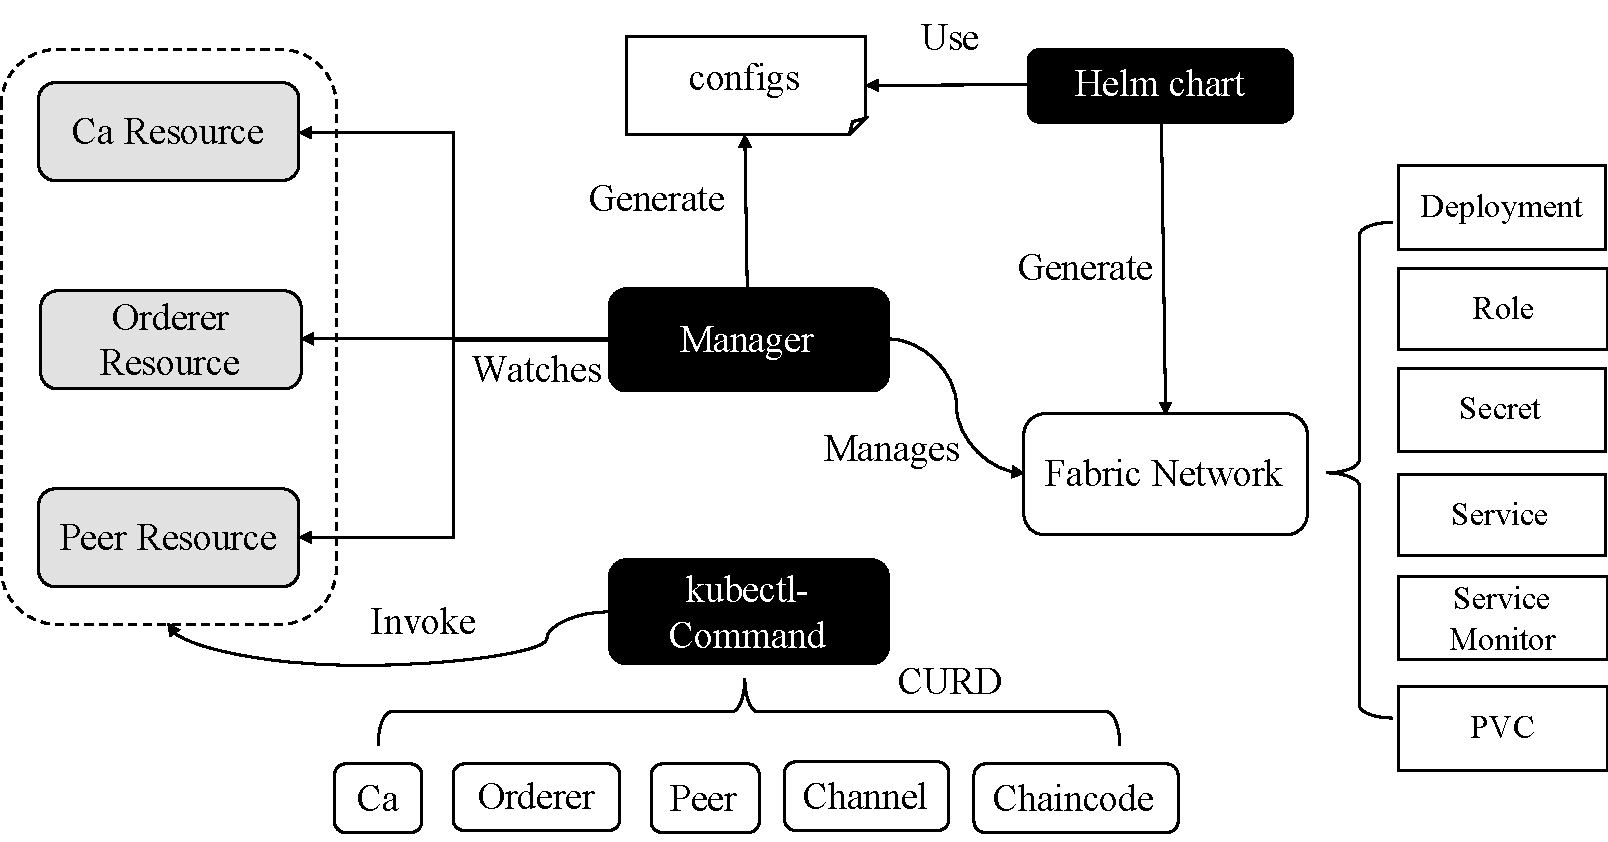
\includegraphics[width=1.0\textwidth]{FIGs/chapter4/framework.pdf} %中括号中的参数是设置图片充满文档的大小,你也可以使用小数来缩小图片的尺寸。
    \caption{基于Hyperledger Fabric的区块链云化框架} %caption是用来给图片加上图题的
    \label{framework} %这是添加标签,方便在文章中引用图片。
\end{figure}%figure环境

\subsection{Custom Resource Definition}\label{section: Custom_Resource_Definition}

CRD通过扩展Kubernetes API将具备领域知识资源类型注入进Kubernetes集群中。Kubernetes提供了标准资源ConfigMap, 也可用于使配置数据项供应用程序使用, 但这两种针对不同的情况。ConfigMap擅长为在集群上的Pod中运行的程序提供配置, 应用程序通常希望从Pod中读取此类配置, 例如文件或环境变量的值, 而不是从Kubernetes API中读取。CRs由标准的Kubernetes客户端创建和访问, 遵守Kubernetes规范。通过自定义controller可以监控CRs运行, 这些代码可以反过来创建、更新或删除其他集群对象, 甚至集群外的任意资源。

Fabric作为一种去中心化的多方信息对接的网络, 具有一套标准化的数据结构与接口。本框架基于Fabric网络各节点自身功能及配置\footnotemark[1]\footnotetext[1]{\href{https://github.com/hyperledger/fabric-ca/blob/main/cmd/fabric-ca-server/config.go}{Ca Config}}\footnotemark[2]\footnotetext[2]{\href{https://github.com/hyperledger/fabric/blob/main/sampleconfig/orderer.yaml}{Orderer Config}}\footnotemark[3]\footnotetext[3]{\href{https://github.com/hyperledger/fabric/blob/main/sampleconfig/core.yaml}{Peer Config}}设计三种Fabric静态资源类型作为输入, 篇幅原因仅展示包括但不限于如表\ref{crd_description}所示的属性。额外的, 除上述针对不同网络节点的特殊属性外, 本框架需要为每个节点提供如副本数、镜像、Hosts、日志、ServiceMonitor等基本属性维持上述网络节点的基本运行状态。

{\footnotesize
\begin{longtable}[h]{m{60pt}|m{100pt}|m{210pt}}
    \caption[CRD描述]{CRD描述} \label{crd_description} \\
        \hline   
        \textbf{CRD名称}&\textbf{属性}&\textbf{描述}\\
        \hline
        \multirow{8}*{\parbox[c]{60pt}{Ca Resource \\ Definition}}
        & CRLSizeLimit & 可接受证书撤销列表(Certificate Revocation List, 简称CRL)的大小限制 \\\cline{2-3}
        & TLS & 服务器侦听TLS端口以及证书等信息 \\\cline{2-3}
        & CA & 包含与证书颁发机构相关的信息 \\\cline{2-3}
        & Database & 用作数据存储 \\\cline{2-3}
        & CFG & 配置身份允许的错误密码尝试次数 \\\cline{2-3}
        & CSR & 控制根CA证书的创建, 如根CA证书的过期时间配置 \\\cline{2-3}
        & Registry & 部分控制fabric-ca服务器执行验证包含用户名和密码的注册和检索标识的属性名称、值的方式 \\\cline{2-3}
        & BCCSP & 用于选择要使用的加密库实现 \\\cline{2-3}
        \hline  
        \multirow{4}*{\parbox[c]{60pt}{Orderer \\ Resource \\ Definition}}
        & Genesis & 初始区块相关配置 \\\cline{2-3}
        & BootstrapMethod & 指定了获取引导块系统通道的方法 \\\cline{2-3}
        & ChannelParticipation & 通道管理对系统链码的依赖 \\\cline{2-3}
        & Secret & 包含Orderer的数字签名以及与Ca通信所需的基本信息\\\cline{2-3}
        \hline 
        \multirow{7}*{\parbox[c]{60pt}{Peer Resource \\ Definition}}
        & Gossip & 确保Peer间通过Gossip协议来达到所有账本的最终一致性 \\\cline{2-3}
        & LevelDB/CouchDB & Fabric提供levelDB与CouchDB用以保存Fabric账本信息, 用以灵活适应Peer不同数据库之间的转换 \\\cline{2-3}
        & CouchDBExporter & 采集CouchDB的监控数据 \\\cline{2-3}
        & ExternalChaincodeBuilder & 提供外部链码构建的能力 \\\cline{2-3}
        & Secret & 包含Peer的数字签名以及与Ca通信所需的基本信息\\\cline{2-3}
        & MSP & 所属的组织信息\\\cline{2-3}
        \hline 
    \end{longtable} 
}

\subsection{Manager}

CRs本身仅为特定应用程序提供声明式API的数据项的集合, controller负责对CRs的不同事件做出反馈, 管理CRs的完整生命周期。

\begin{figure}[h] %figure环境,h默认参数是可以浮动,不是固定在当前位置。如果要不浮动,你就可以使用大写float宏包的H参数,固定图片在当前位置,禁止浮动。
    \centering %使图片居中显示
    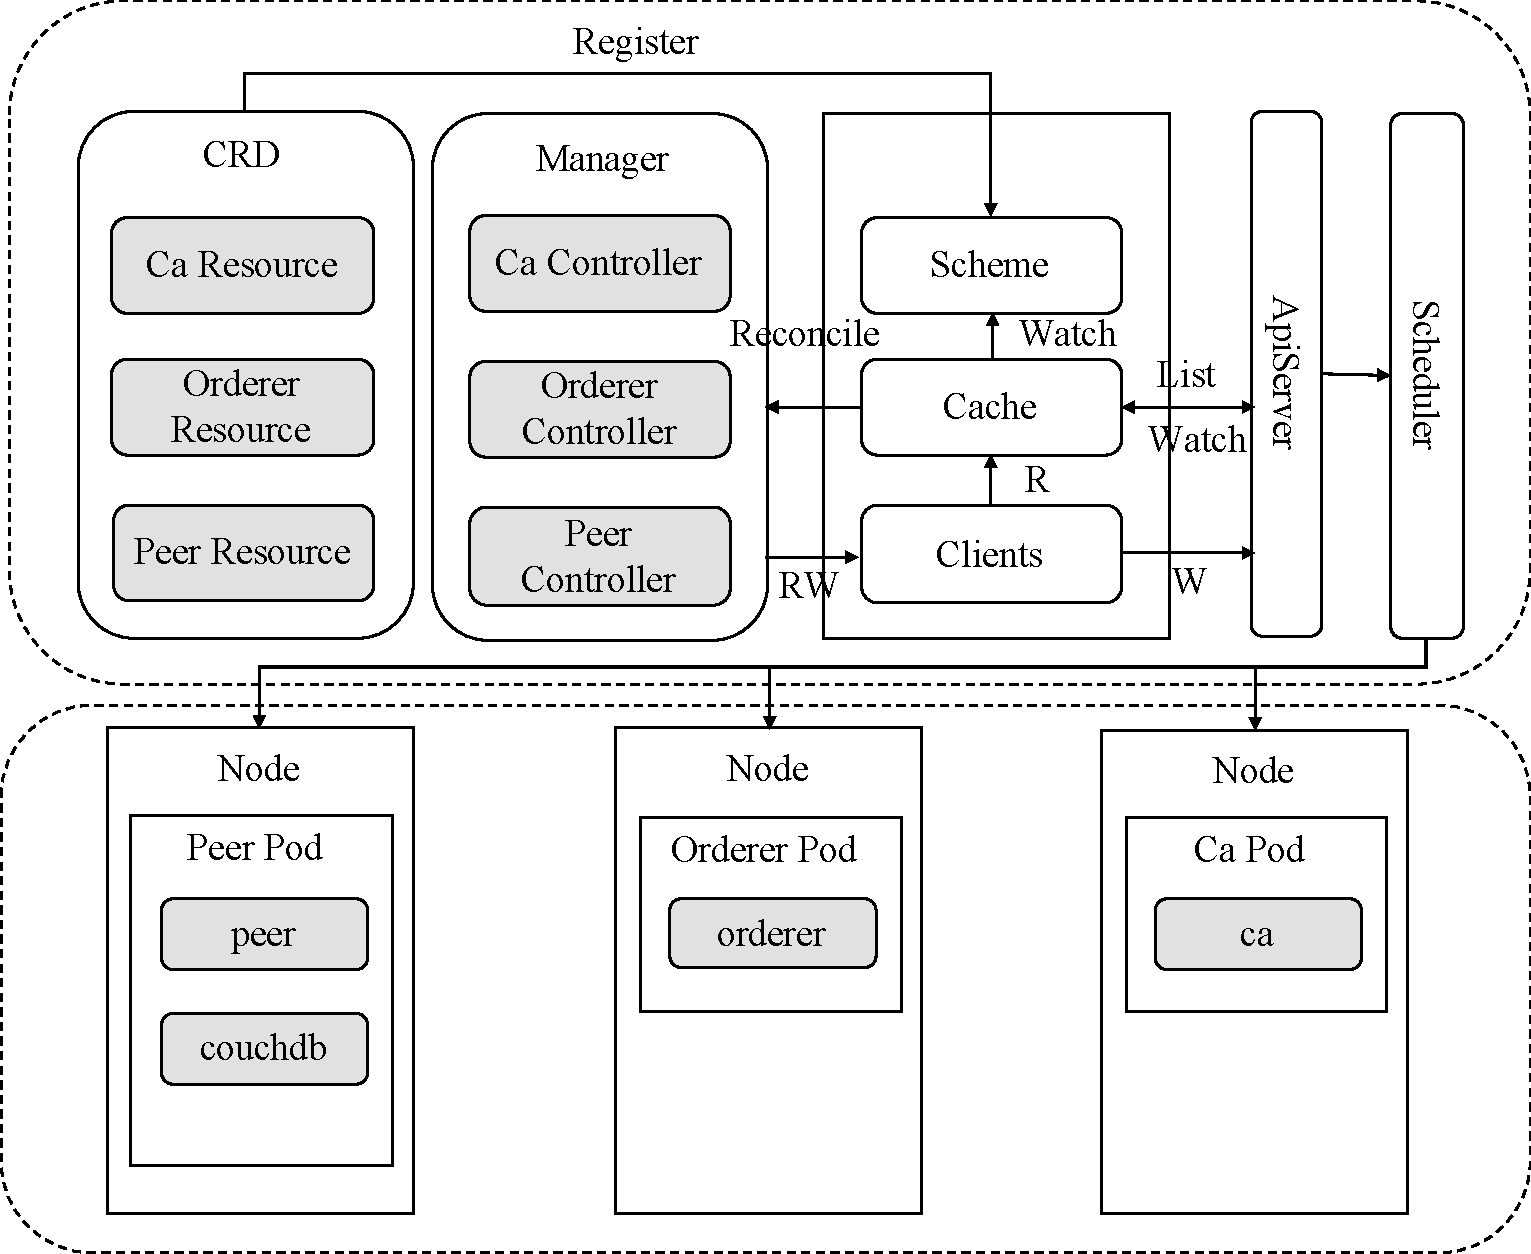
\includegraphics[width=0.95\textwidth]{FIGs/chapter4/manager.pdf} %中括号中的参数是设置图片充满文档的大小,你也可以使用小数来缩小图片的尺寸。
    \caption{Manager监听CRs} %caption是用来给图片加上图题的
    \label{manager} %这是添加标签,方便在文章中引用图片。
\end{figure}%figure环境

在Manager内部管理了多个CRD, 就需要使用多个控制器进行协调循环。这有助于关注点分离和代码的可读性。如图\ref{manager}所展示的是Manager监听CRs的全过程。首先, 需要在CRs中指定Fabric网络各节点所期望的状态, CRD会注册进入Scheme, 其提供了ApiServer对应的集群中GVK(Group Version Kind, Kubernetes集群资源定义方式)与CRs资源类型的映射, 通过资源类型controllers就能获取CRs所定义的期望状态; 其次, cache通过List-Watch机制与ApiServer进行通信用以同步监听Fabric网络各节点在Kubernetes集群中的创建、删除、更新等操作, cache可以获取Fabric网络各节点的实际状态; 最后, controller循环监听期望状态与实际状态, 若期望状态与实际状态不一致, 则通过调用clients更新、缩放、扩展、备份等操作进行协调一致。

为提升区块链云化框架的生产效率, 本文设计了一套针对Fabric网络各节点helm的通用CRD与controller, 直接将提前配置好的helm随CRD以及controller一起部署进Kubernetes。Helm通过调用Kubernetes的ApiServer逐个将helm chart中的yaml推送给Kubernetes, 当且仅能进行安装。所以helm的弊端是缺乏对资源的全生命期监控, 只有CRD才能持续的监听Kubernetes资源对象的变化事件, 进行全生命期的监控响应, 高可靠的完成部署交付。一旦创建新的CR, controller根据对应的资源对象更新helm的模板参数并重新部署入Kubernetes集群。图\ref{controller}以spec.size为例展示了controller更新helm的流程。本框架不仅通过helm简化部署流程, 并且还能实现带全生命周期管理的helm效果。

\begin{figure}[h] %figure环境,h默认参数是可以浮动,不是固定在当前位置。如果要不浮动,你就可以使用大写float宏包的H参数,固定图片在当前位置,禁止浮动。
    \centering %使图片居中显示
    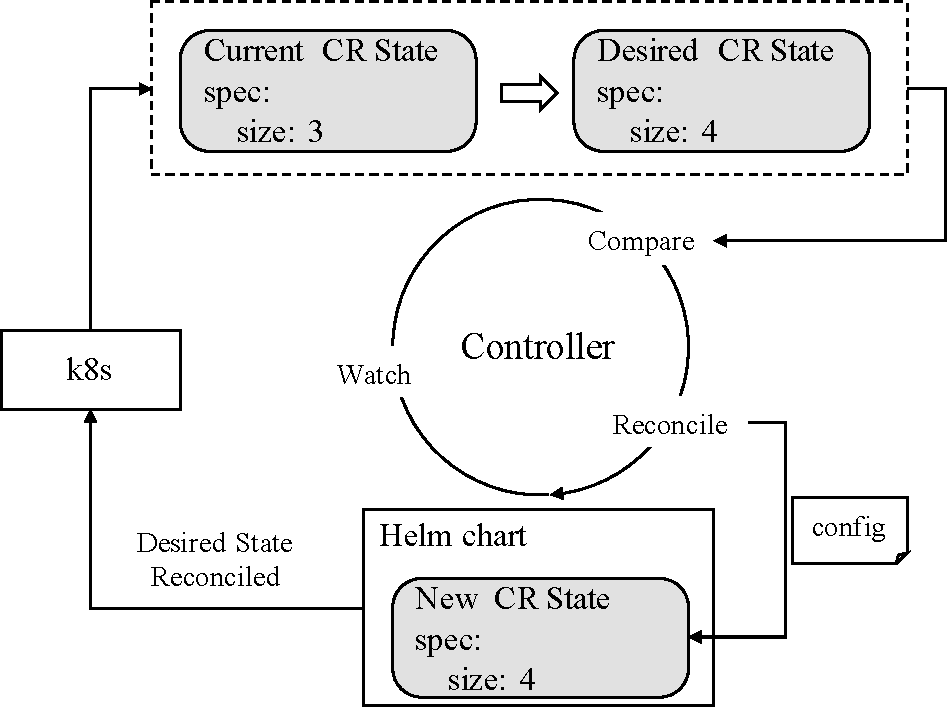
\includegraphics[width=0.75\textwidth]{FIGs/chapter4/controller.pdf} %中括号中的参数是设置图片充满文档的大小,你也可以使用小数来缩小图片的尺寸。
    \caption{controller循环监听} %caption是用来给图片加上图题的
    \label{controller} %这是添加标签,方便在文章中引用图片。
\end{figure}%figure环境

% 可迁移性
区块链云化框架遵循标准化原则, 复用Fabric网络各节点镜像并利用Kubernetes进行编排和管理底层的物理资源。这可以使用户能够轻松地在集群之间移动和部署云化框架及Fabric网络, 确保区块链系统基础架构的云独立性, 取消对云提供商的强依赖性, 提升本框架的的可迁移性与通用性。

% 存储扩展性
除\ref{section: Custom_Resource_Definition}所提到的利用CRD对Fabric网络配置进行模块化设计外, 本框架为每个运行中的Fabric网络节点选择配置的PVC, 并为每个PVC中预留出一定的额外存储资源。相较于对所有持久存储的服务使用一个PVC而言, 虽然分配存储远超必要范围增加额外的存储资源冗余, 但用拥有更对的PVC能够保障每个网络节点拥有足够的存储空间, 以便在不缺乏存储资源的情况下正确运行节点。拥有更多的PVC增加了首次部署难度及过度调配的风险, 但多PVC能够灵活针对不同节点运行情况利用Kubernetes进行有针对性的存储扩容, 增强框架对于存储的扩展性。尽管多PVC在管理方面存在一定的复杂性, 但在选择多PVC更加符合最佳实践, 并且效率更高\cite{d2020design}。
% 可插入图

% 安全性
在安全性方面区块链云化框架复用Kubernetes的原生安全保障体系, 主要涉及到两方面。 一方面是Kubernetes集群用户对框架操作的访问控制限制, 区块链云化框架会生成很多清单文件向Kubernetes集群中部署Fabric网络, 同时Kubernetes集群需要向已部署的区块链云化框架授予在Fabric网络中生命周期内执行各种任务的权限。Kubernetes没有以用户身份进行身份验证, 本框架将所有Fabric网络资源限制在同一命名空间下, 同时采用基于角色的权限控制(Role-Based Access Control, 简称RBAC)将对Kubernetes资源操作的最小权限映射到框架中的Manager及Fabric网络节点。值得注意的是, 区块链云化框架无需以root身份运行, 在确保在允许Fabric网络正常工作的同时, 应尽可能限制访问; 另一方面是Fabric网络运行环境均受Kubernetes安全容器保护。在密码管理方面, 框架避免使用直接向节点镜像中注入环境变量的方式管理密码信息。本框架采用Secret配合x509\cite{8249485}存储管理导出的敏感数据, 这种方式不但能提高灵活性而且增加了密码的传输、存储、访问安全, 增强隐私保护。


% 可视化运维
本框架采用非介入式的云上监控方案Prometheus以及Grafana进行可视运维, 在CRD中预留exporter、ServiceMonitor等属性, 对应的在helm chart中定制抓取周期的相关配置对Fabric网络中的Ca、Orderer、Peer、CouchDB等进行可视化监控。同时, Grafana开源特性能够创建自定义插件, 一定程度上能提升本框架的可视运维能力。


\subsection{Fabric网络}

Fabric网络一个复杂的分布式系统, 需要权衡速度、性能等条件对不同网络节点的部署状态进行合理设计。静态节点Ca、Orderer、Peer在首次启动网络时就需要部署在Kubernetes集群中并以Pod形式运行。Pod是Kubernetes中可以创建和部署的最小单位。在Kubernetes集群中, Pod有两种运行状态:

\begin{itemize}[itemindent=2em]
    \item Pod中运行单容器: 每个Pod一个容器是最常见的状态, 在这种状态下, 可以将Pod当作单容器进行封装, 但Kubernetes管理仍然是Pod而不是容器;

    \item Pod中运行个容器: 当容器间需要紧密协作时可以在同一Pod中运行多容器。
\end{itemize}

Ca是Fabric的证书授权中心, Orderer负责交易的排序, 这两个节点在配置上需要满足可插拔式设计。 但在网络运行时, 需要各自在一个Pod中运行即可, 同时 在一个Pod中运行可以更好的有效的利用Kubernetes的自动缩放功能进行弹性伸缩。

Peer是Fabric中被使用最多的模块, 是Fabric网络的基石, 其负责区块链数据的存储以及运行链码。由于Peer节点需要频繁的账本存储单元如CouchDB进行交互, 所以peer容器应当与couchdb容器存在于同一Pod中。在同一个Pod中, peer容器与couchdb紧密协作, 拥有相同的存活周期, 更优的, 相同Pod中的不同容器共享进程、IP地址和数据卷, 可以进行频繁的文件和数据交换。Peer支持外部链码部署, 即链码拥有自己独立的Pod运行环境与Peer解耦, 能够纳入智能合约微服务化流程\cite{zhangfuli2021smartcontract}进行快速响应与监控。 

\section{原型工具}

\subsection{工具概述}

云原生具有资源按需配置, 动态伸缩的特性。当前, BaaS虽然能够基于云平台构建区块链系统, 但仅提供脚本化的方式部署区块链网络及智能合约, 仍未深入云基础设施平台的底层有效利用云的特性管理区块链平台, 这导致了BaaS平台对云特性的严重浪费。

\begin{figure}[!htbp] %figure环境,h默认参数是可以浮动,不是固定在当前位置。如果要不浮动,你就可以使用大写float宏包的H参数,固定图片在当前位置,禁止浮动。
    \centering %使图片居中显示
    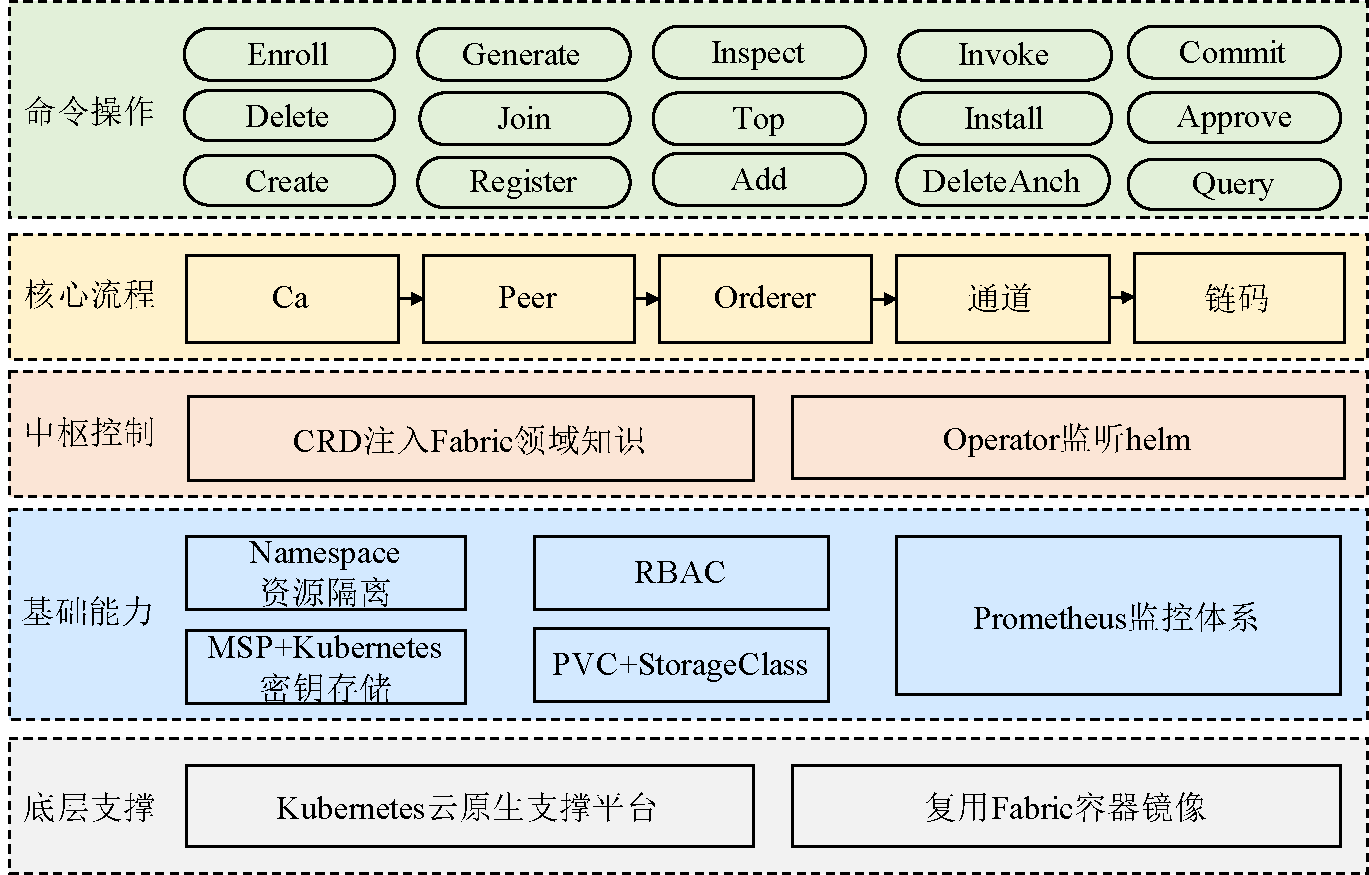
\includegraphics[width=1.0\textwidth]{FIGs/chapter4/tool.pdf} %中括号中的参数是设置图片充满文档的大小,你也可以使用小数来缩小图片的尺寸。
    \caption{原型工具总体功能} %caption是用来给图片加上图题的
    \label{toolstotal} %这是添加标签,方便在文章中引用图片。
\end{figure}%figure环境

因此, 一个支持区块链有效云化的工具十分重要。如图\ref{toolstotal}所示, 本文基于提出区块链云化框架提供配套的基于Hyperledger Fabric的区块链云化原型工具。原型工具建立在Fabric核心流程之上, 对外不仅完成以声明式的方式自动化配置Fabri网络中的Ca、Orderer、Peer实体组件而且能够以命令的方式动态管理整个Fabric网络, 包含静态Fabric组件以及通道、链码的全生命周期管理; 对内应当区块链领域知识注入进云平台Kubernetes中, 有效利用Kubernetes的安全性、数据扩展性、可监控等能力为Fabric网络赋能。



\subsection{需求分析}

\subsubsection{功能性需求分析}

\begin{figure}[!htbp] %figure环境,h默认参数是可以浮动,不是固定在当前位置。如果要不浮动,你就可以使用大写float宏包的H参数,固定图片在当前位置,禁止浮动。
    \centering %使图片居中显示
    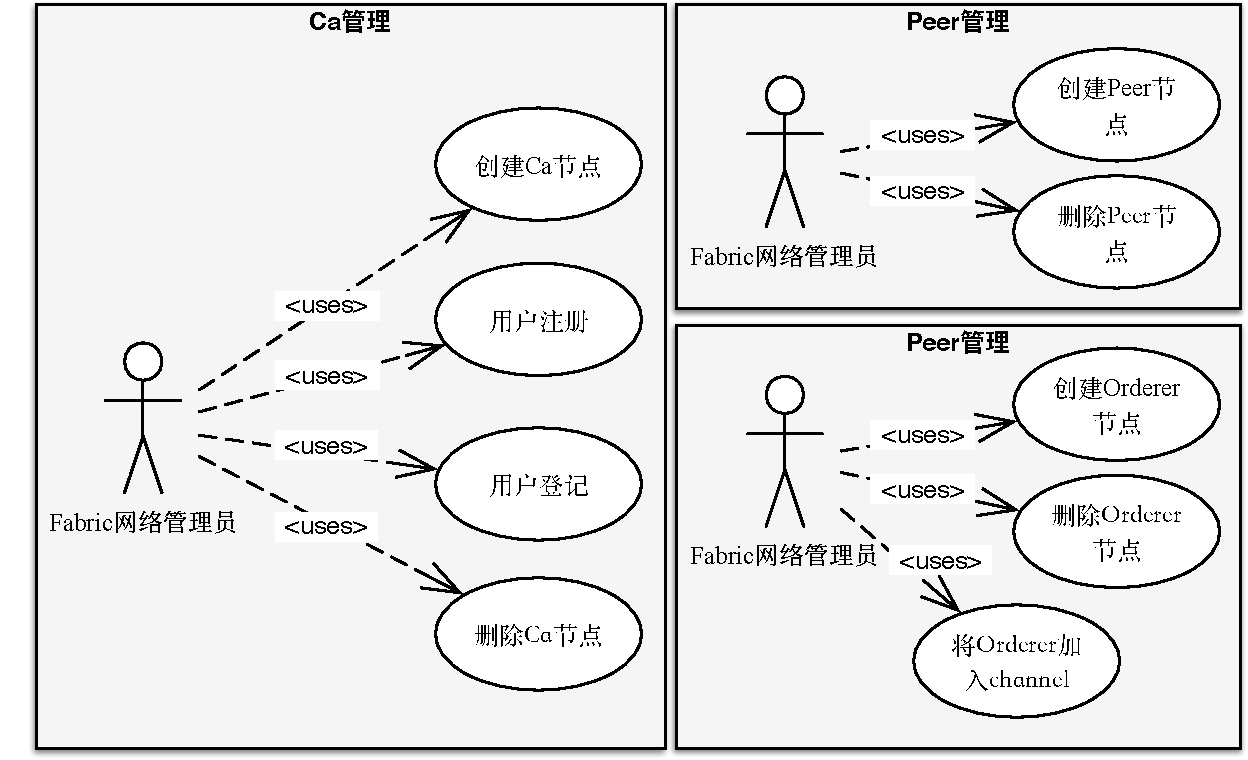
\includegraphics[width=1.0\textwidth]{FIGs/chapter4/fabric_use_case.pdf} %中括号中的参数是设置图片充满文档的大小,你也可以使用小数来缩小图片的尺寸。
    \caption{Fabric网络管理用例图} %caption是用来给图片加上图题的
    \label{fabric_use_case} %这是添加标签,方便在文章中引用图片。
\end{figure}%figure环境


如图\ref{fabric_use_case}所示, Fabric网络管理人员期望能够通过原型工具不影响原节点功能性的前提下对Fabric网络各节点分别进行命令式启停, 降低Fabric网络的启动时间成本。


% 注册->进数据库->签发证书->生成证书文件

表\ref{ca_use_case}展示了Ca管理的用例描述, Ca管理需为Fabric网络管理人员提供灵活方便的启停Ca节点的功能, 同时提供管理注册、签发证书的功能。在启动过程中应以kubectl内置命令行参数配置的方式设置Ca启动所可选的配置项, 如Database、Host、CLRSizeLimit等。同样, Ca管理需要覆盖Ca节点原有基本的用户注册、用户登记的功能。

{\footnotesize
\begin{longtable}[h]{m{60pt}|m{280pt}}
    \caption[Ca管理用例表]{Ca管理用例表} \label{ca_use_case} \\
        \hline  
        ID&UC-Ca\\
        \hline
        名称&可视化建模用例\\
        \hline
        描述&Fabric网络管理员可以通过kubectl的方式创建、删除Ca节点, 并能够以命令行参数的形式将Ca启动参数注入。 同时, Fabric网络管理员能够无障碍进行用户注册、登记。\\
        \hline
        触发条件&Fabric网络管理员输入对应Ca命令\\
        \hline
        前置条件&Kubernetes集群环境\\
        \hline
        后置条件&无\\
        \hline
        正常流程& (1)Fabric网络管理员输入“kubectl-hlf ca create”并以可选参数的形式输入其他如Ca名称、容量等配置项;
        \newline (2)Fabric网络管理员输入“kubectl-hlf ca register”并以可选参数的形式输入其他如用户名、密码等配置项;
        \newline (3)Fabric网络管理员输入“kubectl-hlf ca enroll”并输入已经注册过的用户名、密码等信息将注册的用户进行登记并导出证书信息;
        \newline (4)可选的, Fabric网络管理员输入“kubectl-hlf ca delete”并输入ca-name以删除ca节点;\\
        \hline
        异常流程&无\\
        \hline
    \end{longtable} 
}


表\ref{peer_use_case}展示了Peer管理的用例描述, Peer管理需为Fabric网络管理人员提供灵活方便的启停Peer节点的功能, 在启动过程中应以kubectl内置命令行参数配置的方式设置Peer启动所可选的配置项, 如Peer对应的Ca名称账本存储类型、Gossip协议、组织信息等。

{\footnotesize
\begin{longtable}[h]{m{60pt}|m{280pt}}
    \caption[Peer管理用例表]{Peer管理用例表} \label{peer_use_case} \\
        \hline  
        ID&UC-Peer\\
        \hline
        名称&可视化建模用例\\
        \hline
        描述&Fabric网络管理员可以通过kubectl的方式创建、删除Peer节点, 并能够以命令行参数的形式将Peer启动参数注入。\\
        \hline
        触发条件&Fabric网络管理员输入对应Peer命令\\
        \hline
        前置条件&已经启动对应组织级的Ca\\
        \hline
        后置条件&无\\
        \hline
        正常流程& (1)Fabric网络管理员输入“kubectl-hlf peer create”并以可选参数的形式输入其他如Peer名称、所属组织、账本存储类型等配置项;
        \newline (2)可选的, Fabric网络管理员输入“kubectl-hlf peer delete”并输入peer-name以删除Peer节点;\\
        \hline
        异常流程& Fabric网络管理员输入的对应Ca名称匹配不上, 报错提示\\
        \hline
    \end{longtable} 
}

表\ref{orderer_use_case}展示了Orderer管理的用例描述, Orderer管理需为Fabric网络管理人员提供灵活方便的启停Orderer节点的功能, 同时能够将Orderer加入到通道中,在启动过程中应以kubectl内置命令行参数配置的方式设置Orderer启动所可选的配置项, 如Orderer对应的Ca名称、自己的名称、组织、容量等信息。

{\footnotesize
\begin{longtable}[h]{m{60pt}|m{280pt}}
    \caption[Orderer管理用例表]{Orderer管理用例表} \label{orderer_use_case} \\
        \hline  
        ID&UC-Orderer\\
        \hline
        名称&可视化建模用例\\
        \hline
        描述&Fabric网络管理员可以通过kubectl的方式创建、删除Orderer节点, 并能够以命令行参数的形式将Orderer启动参数注入。\\
        \hline
        触发条件&Fabric网络管理员输入对应Orderer命令\\
        \hline
        前置条件& (1)已经启动对应组织级的Ca
        \newline (2)Orderer加入通道前确保通道建立\\
        \hline
        后置条件&无\\
        \hline
        正常流程& (1)Fabric网络管理员输入“kubectl-hlf ordnode create”并以可选参数的形式输入其他如Orderer名称、所属组织、所属组织的Ca名称等配置项;
        \newline (2)Fabric网络管理员输入“kubectl-hlf ordnode join” 并以参数的形式输入名称、命名空间、输入创世区块信息、自己的证书文件;
        \newline (3)可选的, Fabric网络管理员输入“kubectl-hlf ordnode delete”并输入orderer-name以删除Orderer节点;\\
        \hline 
        异常流程& (1) Fabric网络管理员输入的对应Ca名称匹配不上, 报错提示;
        \newline (2) Orderer节点证书文件验证不通过, 禁止加入; \\
        \hline
    \end{longtable} 
}

\begin{figure}[!htbp] %figure环境,h默认参数是可以浮动,不是固定在当前位置。如果要不浮动,你就可以使用大写float宏包的H参数,固定图片在当前位置,禁止浮动。
    \centering %使图片居中显示
    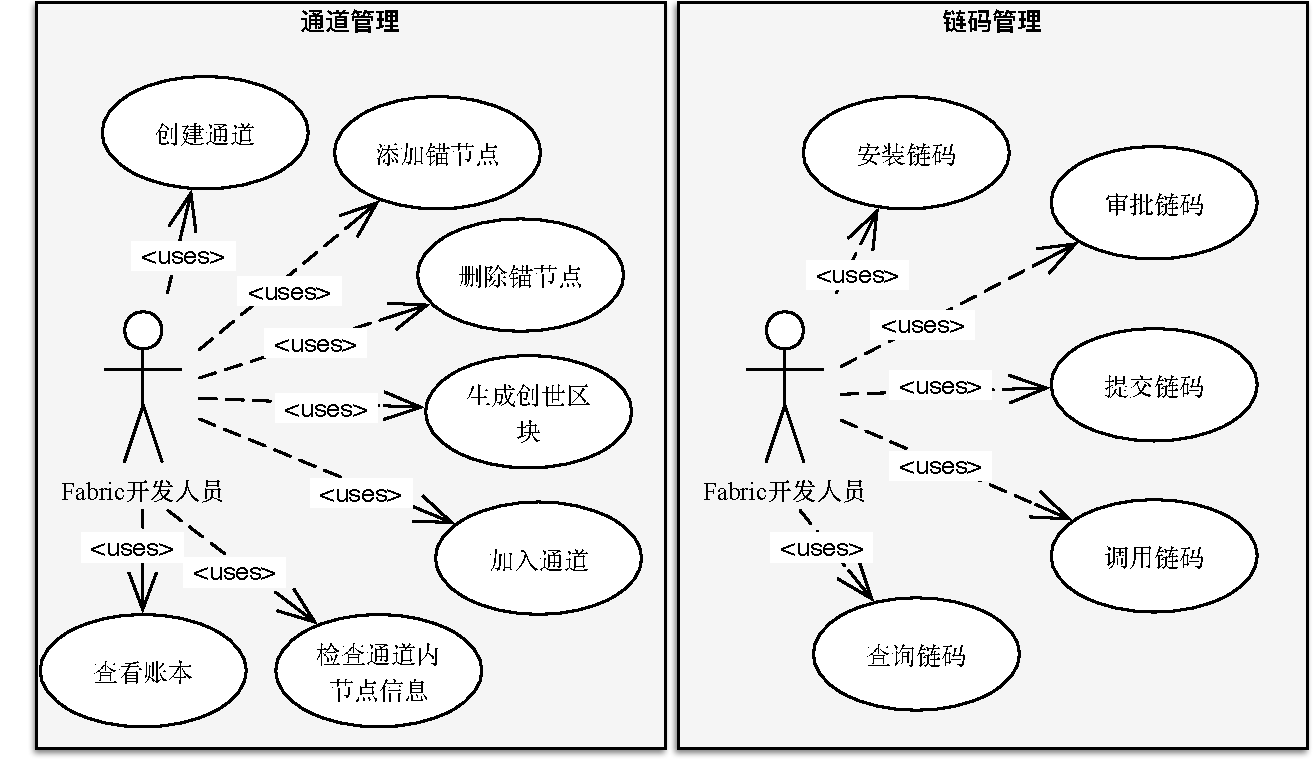
\includegraphics[width=1.0\textwidth]{FIGs/chapter4/chan_cc_use_case.pdf} %中括号中的参数是设置图片充满文档的大小,你也可以使用小数来缩小图片的尺寸。
    \caption{通道管理及链码管理用例图} %caption是用来给图片加上图题的
    \label{chan_cc_use_case} %这是添加标签,方便在文章中引用图片。
\end{figure}%figure环境


{\footnotesize
\begin{longtable}[h]{m{60pt}|m{280pt}}
    \caption[通道管理用例表]{通道管理用例表} \label{chan_use_case} \\
        \hline  
        ID&UC-Orderer\\
        \hline
        名称&可视化建模用例\\
        \hline
        描述&Fabric开发人员可以通过kubectl的方式创建、管理通道\\
        \hline
        触发条件&Fabric网络管理员输入对应通道命令\\
        \hline
        前置条件&已经启动好基础Fabric网络, 包含Ca、Orderer、Peer\\
        \hline
        后置条件&无\\
        \hline
        正常流程& (1)Fabric开发人员输入“kubectl-hlf channel generate”并以可选参数的形式输入所包含的组织名称以及输出的创世区块保存文件;
        \newline (2)Fabric开发人员输入“kubectl-hlf channel join” 并以参数的形式输入应当加入该通道的节点名称、组织信息和用户;
        \newline (3)Fabric开发人员员输入“kubectl-hlf channel inspect”并以参数的形式输入通道的名称导出该通道内配置与Orderer、Peer节点的信息;
        \newline (4)Fabric开发人员员输入“kubectl-hlf channel addanchorpeer”并以参数的形式输入通道的名称用以向通道中加入锚节点;
        \newline (5)Fabric开发人员员输入“kubectl-hlf channel top”并以参数的形式输入通道的名称用以向查询账本的高度;\\
        \hline 
        异常流程& 无; \\
        \hline
    \end{longtable} 
}

{\footnotesize
\begin{longtable}[h]{m{60pt}|m{280pt}}
    \caption[链码管理用例表]{链码管理用例表} \label{cc_use_case} \\
        \hline  
        ID&UC-Orderer\\
        \hline
        名称&可视化建模用例\\
        \hline
        描述&Fabric开发人员可以通过kubectl的方式安装、提交、查询链码;\\
        \hline
        触发条件&Fabric开发人员输入对应链码命令\\
        \hline
        前置条件&已经部署好通道\\
        \hline
        后置条件&无\\
        \hline
        正常流程& (1)Fabric开发人员输入“kubectl-hlf chaincode intall”并以可选参数的形式输入链码所在地址、链码语言、标签等参数用以安装链码;
        \newline (2)Fabric开发人员输入“kubectl-hlf chaincode queryinstalled" 并以参数的形式传入组织名称、用户、Peer信息等参数用以展示已经安装的链码;
         \newline (3)Fabric开发人员输入“kubectl-hlf chaincode approveformyorg" 并以参数的形式传入链码package-id、链码名称、组织信息、策略等参数用以所在组织审批链码;
        \newline (4)Fabric开发人员输入“kubectl-hlf chaincode commit”并以参数的形式输入链码名称、策略等信息用以提交链码
        \newline (5)Fabric开发人员输入“kubectl-hlf chaincode invoke”并以参数的形式输入链码名称、调用方法等信息用以调用链码
        \newline (6)Fabric开发人员输入“kubectl-hlf chaincode query”并以参数的形式输入链码名称、调用方法等信息用以查询链码\\
        \hline 
        异常流程& (1)因网络原因安装链码时间过长而导致, 提示并报错\\
        \hline
    \end{longtable} 
}

除管理Fabric网络节点外, 如图\ref{chan_cc_use_case}所示, Fabric开发人员期望能够通过原型工具
动态、灵活且低成本的完成通道以及链码的各项操作。

表\ref{chan_use_case}展示了通道管理的用例描述, 通道管理需为Fabric开发人员屏蔽大量证书文件提供灵活方便的开启通道的功能, 应以kubectl内置命令行参数配置的方式在配置通道, 包含对通道内部锚节点、创世区块、账本的管理。表\ref{cc_use_case}展示了链码管理的用例描述, 链码管理需为Fabric网络管理人员提供灵活方便的安装、提交链码等功能。


\subsubsection{非功能性需求分析}

本文涉及的区块链云化框架原型工具需要为Fabric网络及链码提供标准化的、便捷化启停构建方式, 同时还需要利用云的特性提升以下非功能性需求:

\begin{itemize}[itemindent=2em]
    \item 易用性: Fabric网络管理人员和开发人员在学习了基本的Fabric概念之后且Fabric网络组件镜像完备的情况下, 可以通过原型工具简化Fabric网络配置流程并应当在10分钟之内完成Fabric网络的构建;

    \item 可迁移性: 原型工具需要具备便捷的安装方式, 以便于能够在支持Kubernetes的云上自由迁移;

    \item 可扩展性: 原型工具需要为Fabric网络提供可插拔的标准化接口, 如共识算法、账本存储单元等; 同时, 随着交易数量的增加, 链外存储压力上升, 工具应能对存储进行动态的不重启扩容;

    \item 安全性: 原型工具需要具备严格的权限访问控制策略, Fabric网络管理员(开发人员)需要经过认证之后才能有权限操作Fabric网络各节点的启停; 只有经过认证的Fabric网络用户才能进行合法交易;

    \item 可靠性: 在命令输入过程中, 原型工具应当提前自动校验命令行参数的准确性, 能够判断各种异常输入并快速做出提示响应, 防止出现异常;

\end{itemize}


\subsection{设计与实现}

基于Hyperledger Fabric的区块链云化工具是一个基于Kubernetes operator的应用, 其整合结合Helm完成Fabric网络的快速部署和节点的全生命周期管理以及Cobra\footnotemark[1]\footnotetext[1]{\href{https://github.com/spf13/cobra}{cobra github地址}}完成命令的封装。由于原型工具在管理Ca、Orderer、Peer各组件时存在逻辑上的重复性, 故本节将以Ca为例介绍功能性需求、非功能性需求的设计与实现。

% create CRD
当Fabric网络管理员需要创建Ca并输入对应的命令及参数时, 如图\ref{create_crd}。原型工具首先会解析管理员输入参数的合法性, 然后将对应的输入参数填充到已经定义好的FabricCA模版中,最后调用Kubernetes client将Fabric Ca Resource依据CRD的规则部署进入集群中。伪代码\ref{code1}展示了创建Ca Resource的伪代码。

\begin{figure}[!htbp] %figure环境,h默认参数是可以浮动,不是固定在当前位置。如果要不浮动,你就可以使用大写float宏包的H参数,固定图片在当前位置,禁止浮动。
    \centering %使图片居中显示
    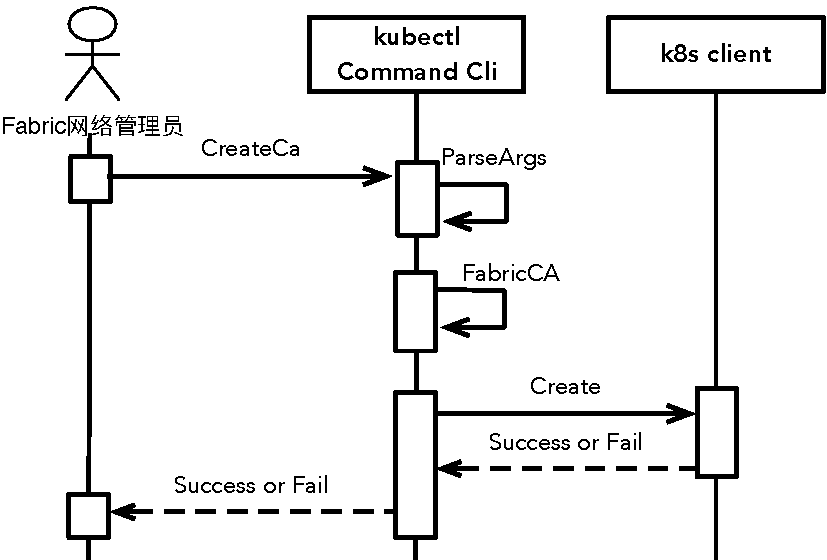
\includegraphics[width=0.7\textwidth]{FIGs/chapter4/create_crd.pdf} %中括号中的参数是设置图片充满文档的大小,你也可以使用小数来缩小图片的尺寸。
    \caption{创建Ca Resource时序图} %caption是用来给图片加上图题的
    \label{create_crd} %这是添加标签,方便在文章中引用图片。
\end{figure}%figure环境

\begin{algorithm}[!htbp]
    \floatname{algorithm}{\footnotesize 伪代码}
    \caption{\footnotesize 创建Ca Resource伪代码}
    \label{code1}
    {\footnotesize
    \begin{algorithmic}
        \renewcommand{\algorithmicrequire}{ \textbf{Input:}}
        \REQUIRE  
        “kubeclt ca create” with args

        \renewcommand{\algorithmicensure}{\textbf{Output:}}
        \ENSURE
        Success or Fail

        \STATE{err := ParseArgs()}
        \IF{err != nil}
            \STATE{return fail} 
        \ENDIF

        \STATE{client, err  := GetKubeOperatorClient()}
        \IF{err != nil}
            \STATE{return fail} 
        \ENDIF

        \STATE{fabricCa := \&v1alpha1.FabricCA\{}
        \STATE{\quad Initialization according to parameters}
        \STATE{\}}


        \IF{args.output}
            \STATE{out, err := yaml.Marshal(\&fabricCa)} 
        \ELSE
            \STATE{err := client.FabricCA(namespaces).Create(fabricCa)}
            \IF{err != nil}
                \STATE{return fail} 
            \ENDIF
        \ENDIF

        \STATE{return success}
    \end{algorithmic}
    }
\end{algorithm}

当Fabric Ca Resource一旦被部署到集群中就会被处理单元Manager中的Ca  controller探查到其存活。如图\ref{reconcile}所示, Ca controller通过Reconcile循环探听Ca Resource。由于资源被删除后再也无法获取到被删除资源的信息, 所以利用Finalizer字段进行标识, GetDeletetionTimeStamp()用于获取CR被删除时的时间戳。一旦探听到Ca Resource的存在就会先处理Finalizer字段。DeletionTimestamp不为空时, controller会轮询该CR的更新请求执行处理所有的Finalizer。随后, Ca controller会检查当前是否存在Ca helm release, 若不存在则将当前状态Ca Resource所定义的TLS、CFG等信息生成helm chart并将其部署进入集群中; 若存在则先获取当前Ca Resource的状态并对其进行更新之后再生成helm chart部署。helm chart中定义了Ca启动所需要的全部如Deployment、Service、Istio、ServiceMonitor等yaml, 通过启动helm就可以一次性将其全部启动部署。伪代码\ref{code2}展示了Ca Controller Reconcile的伪代码。


% Manager
\begin{figure}[!htbp] %figure环境,h默认参数是可以浮动,不是固定在当前位置。如果要不浮动,你就可以使用大写float宏包的H参数,固定图片在当前位置,禁止浮动。
    \centering %使图片居中显示
    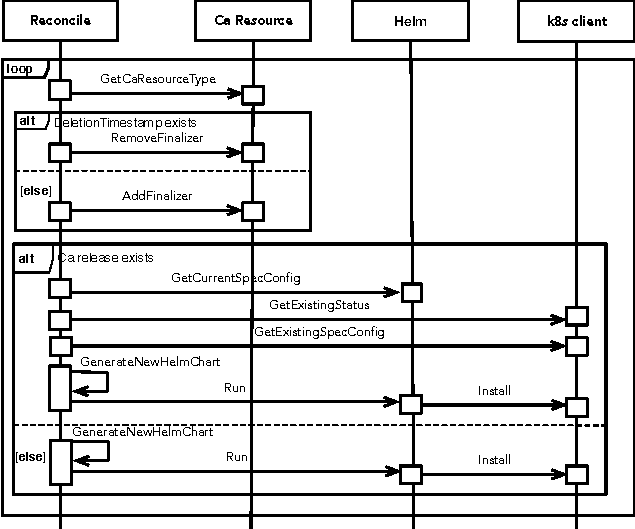
\includegraphics[width=1.0\textwidth]{FIGs/chapter4/reconcile.pdf} %中括号中的参数是设置图片充满文档的大小,你也可以使用小数来缩小图片的尺寸。
    \caption{Ca Controller Reconcile逻辑时序图} %caption是用来给图片加上图题的
    \label{reconcile} %这是添加标签,方便在文章中引用图片。
\end{figure}%figure环境


\begin{algorithm}[!htbp]
    \floatname{algorithm}{\footnotesize 伪代码}
    \caption{\footnotesize Ca Controller Reconcile伪代码}
    \label{code2}
    {\footnotesize
    \begin{algorithmic}
        \renewcommand{\algorithmicrequire}{ \textbf{Input:}}
        \REQUIRE  
        nil

        \renewcommand{\algorithmicensure}{\textbf{Output:}}
        \ENSURE
        nil

        \STATE{fabricCa := \&v1alpha1.FabricCA\{\}}
        \IF{fabricCa.GetDeletetionTimestamp() != nil}
            \IF{fabricCa.GetFinalizers().contains(caFinalizer)}
                \STATE{RemoveFinalizer(fabricCa, caFinalizer)} 
            \ENDIF
        \ENDIF

        \IF{!fabricCa.GetFinalizers().contains(caFinalizer)}
            \STATE{AddFinalizer(fabricCa, caFinalizer)} 
        \ENDIF

        \STATE{exits, err  := status.Run(caReleaseName)}
        \IF{err != nil}
            \STATE{return err} 
        \ENDIF

        \IF{exits}
            \STATE{c, err := GetCurrentSpecConfig(caReleaseName)}
            \IF{err != nil}
                \STATE{return err} 
            \ENDIF
            \STATE{s, err := GetExistingStatus(caReleaseName)}
            \IF{err != nil}
                \STATE{return err} 
            \ENDIF
            \STATE{newCa := fabricCa.DeepCopy()}
            \STATE{newCa.Status = s.Status}

            \STATE{release, err  := cmd.Run(caReleaseName, c)}
            \IF{!reflect.DeepEqual(newCa.Status, release.Status)}
                \STATE{\_, err := status().Update(newCa)}
                \IF{err != nil}
                    \STATE{return err} 
                \ENDIF
            \ENDIF 
            
        \ELSE
            \STATE{c, err := GetCurrentSpecConfig(caReleaseName)}
            \IF{err != nil}
                \STATE{return err} 
            \ENDIF
            \STATE{release, err  := cmd.Run(caReleaseName, c)}
            \IF{err != nil}
                \STATE{return err} 
            \ENDIF

        \ENDIF
      
    \end{algorithmic}
    }
\end{algorithm}

当Ca成功在Kubernetes中启动后, 可以通过命令形式完成用户注册、用户登记的功能。如图\ref{enroll}所示, Fabric网络管理员输入Enroll命令以及相关参数, 原型工具会对其进行参数解析。当解析成功后, 原型工具会获取集群中Ca对外接口的相关信息, 包含URL、端口等。随后, 原型工具会生成Ca client, 并将管理员输入的用户信息通过接口传递给Ca Server。Ca Server就是原Fabric Ca在集群中服务的状态所以其具备完整的Ca的功能, 当Enroll完成后会返回key以及cert, 原型工具会利用X509对其编码并保存到yaml中返回给管理员。伪代码\ref{code3}展示了Ca Enroll User的伪代码。

% Manager
\begin{figure}[!htbp] %figure环境,h默认参数是可以浮动,不是固定在当前位置。如果要不浮动,你就可以使用大写float宏包的H参数,固定图片在当前位置,禁止浮动。
    \centering %使图片居中显示
    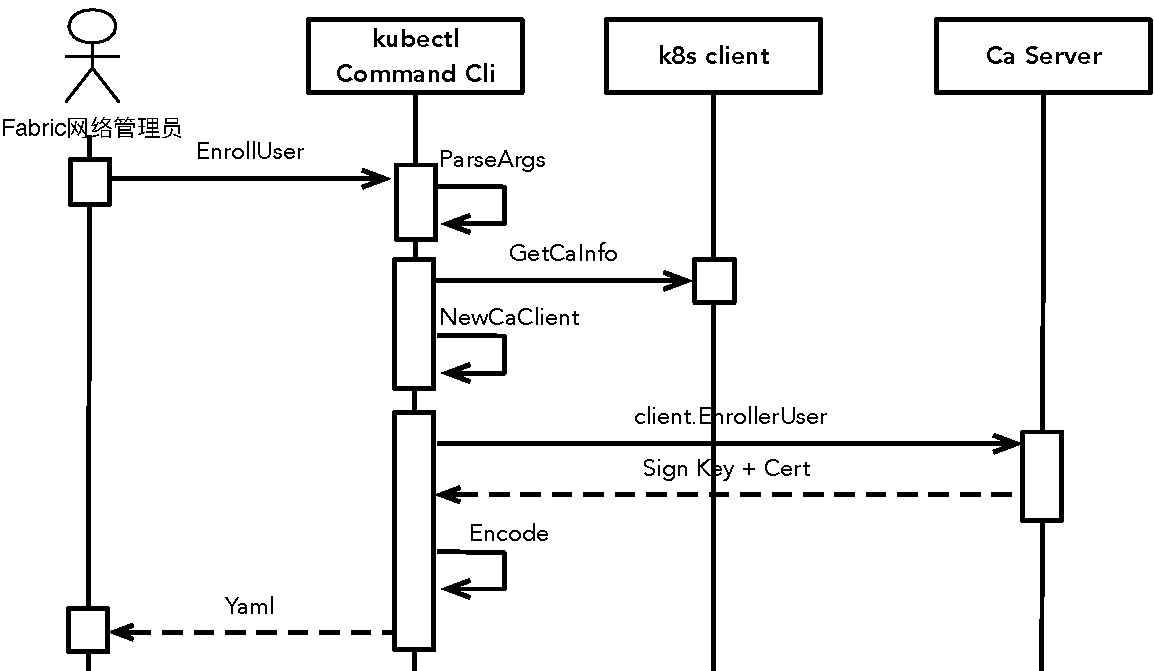
\includegraphics[width=1.0\textwidth]{FIGs/chapter4/enroll.pdf} %中括号中的参数是设置图片充满文档的大小,你也可以使用小数来缩小图片的尺寸。
    \caption{Ca Enroll User逻辑时序图} %caption是用来给图片加上图题的
    \label{enroll} %这是添加标签,方便在文章中引用图片。
\end{figure}%figure环境

\begin{algorithm}[!htbp]
    \floatname{algorithm}{\footnotesize 伪代码}
    \caption{\footnotesize Ca Enroll User伪代码}
    \label{code3}
    {\footnotesize
    \begin{algorithmic}
        \renewcommand{\algorithmicrequire}{ \textbf{Input:}}
        \REQUIRE  
        “kubeclt ca enroll” with args

        \renewcommand{\algorithmicensure}{\textbf{Output:}}
        \ENSURE
        User key\&cert yaml

        \STATE{err := ParseArgs()}
        \IF{err != nil}
            \STATE{return fail} 
        \ENDIF

        \STATE{client, err  := GetKubeOperatorClient()}
        \IF{err != nil}
            \STATE{return fail} 
        \ENDIF

        \STATE{url, err  := GetURLForCa()}
        \IF{err != nil}
            \STATE{return fail} 
        \ENDIF

        \STATE{crt, pk , err:= client.EnrollUser(args.Name, args.Secret, url)}

        \IF{err != nil}
            \STATE{return fail} 
        \ENDIF
 
        \STATE{crtPem := EncodeX509Certificate(crt)}
        \STATE{pkPem := EncodePrivateKey(pk)}

        \STATE{userYaml := yaml.Marshal(\{}
        \STATE{\quad "key": pkPem,} 
        \STATE{\quad "cert": crtPem} 
        \STATE{\})}

        \STATE{io.writeFile(args.output, userYaml)}

        \STATE{return nil}
    \end{algorithmic}
    }
\end{algorithm}

原型工具为Fabric网络的各组件提供了标准化的helm chart模板。除Deployment以及Service外, 在访问权限控制方面采用RBAC的方式。原型工具将所有资源放入同一命名空间下, 对于自定义生成的资源, 设置了两种类型的角色(ClusterRole)分别是editor以及viewer, 如图\ref{safety}-I展示了viewer角色的权限, editor相较于viewer则增加了create、delete、update、patch的权限, 使用ClusterRoleBinding将角色与用户(ServiceAccount)进行捆绑。如图\ref{safety}-II所示, 原型工具通过Secret保存Fabric网络生成的敏感密钥数据。

\begin{figure}[h] %figure环境,h默认参数是可以浮动,不是固定在当前位置。如果要不浮动,你就可以使用大写float宏包的H参数,固定图片在当前位置,禁止浮动。
    \centering %使图片居中显示
    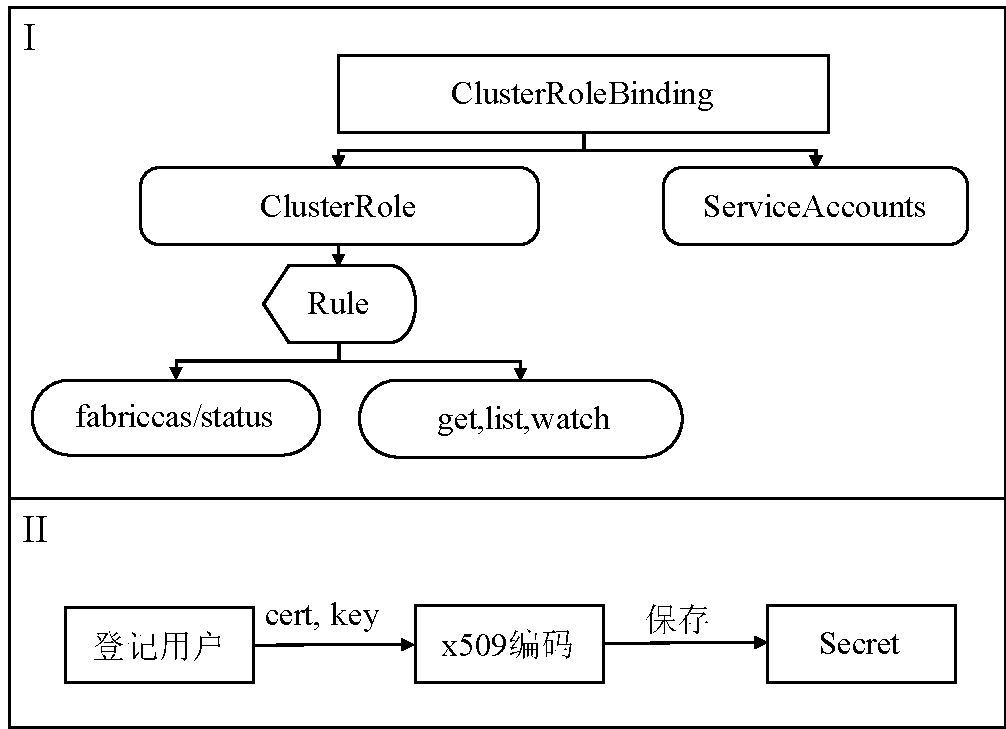
\includegraphics[width=0.8\textwidth]{FIGs/chapter4/safety.pdf} %中括号中的参数是设置图片充满文档的大小,你也可以使用小数来缩小图片的尺寸。
    \caption{原型工具安全策略} %caption是用来给图片加上图题的
    \label{safety} %这是添加标签,方便在文章中引用图片。
\end{figure}%figure环境

在数据存储扩容方面, 原型工具采用链外存储的方式, 利用PVC及StorageClass动态资源供应模式将交易数据高效的写入可插拔式的持续久化介质里面。如图\ref{pvc_sc}所示, 当Fabric网络管理员创建Peer节点并输入需要多少容量的couchDB时, 原型工具会根据内置的PVC进行适配寻找合适的PV进行存储。PVC只是针对于存储的声明并不会进行真正的存储, 其服务于Peer Pod。原型工具在启动初期会定义StorageClass供PVC使用, 当新的Pod PVC被创建时, Kubernetes会寻找StorageClass并为PVC创建符合要求的PV以供存储。原型工具在定义StorageClass时会将“allowVolumeExpansion”字段设置为“true”, 当Fabric网络管理员设定的初始存储值不够时, 可以通过修改PVC的容量进行动态的灵活扩容。链外存储的使得账本数据与操作独立实现, “账本数据生于链却独立于链”, 能够更好的支持数据治理。

\begin{figure}[h] %figure环境,h默认参数是可以浮动,不是固定在当前位置。如果要不浮动,你就可以使用大写float宏包的H参数,固定图片在当前位置,禁止浮动。
    \centering %使图片居中显示
    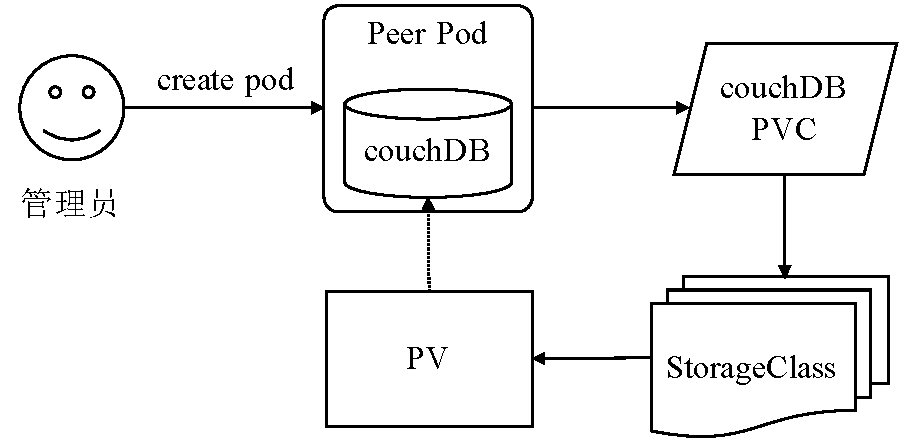
\includegraphics[width=0.7\textwidth]{FIGs/chapter4/pvc_sc.pdf} %中括号中的参数是设置图片充满文档的大小,你也可以使用小数来缩小图片的尺寸。
    \caption{原型工具存储策略} %caption是用来给图片加上图题的
    \label{pvc_sc} %这是添加标签,方便在文章中引用图片。
\end{figure}%figure环境

最后, 原型工具利用Prometheus监控体系给所有Fabric网络组件以及工具本身提供监控能力。利用Prometheus并在Helm chart中配置ServiceMonitor、PodMonitor可以为监控对象实时采集数据并存储。 此外, 搭配Grafna提供可视化面板方便对Fabric网络各项指标进行监控。

\section{本章小节}

本章介绍了基于Hyperledger Fabric的区块链云化框架及其原型工具。首先, 根据\ref{section: policy_set_application}所得的策略具体实施方案给出了云化框架的云化框架的工作流程、输入单元CRD、处理单元Manager以及输出单元Fabric网络节点运行状态。然后结合云化框架介绍了搭配原型工具的需求分析、设计与实现。



% \begin{algorithm}[!htbp]
%     \floatname{algorithm}{\footnotesize 算法}
%     \caption{\footnotesize 模型校验算法}
%     \label{algorithm1}
%     {\footnotesize
%     \begin{algorithmic}
%         \renewcommand{\algorithmicrequire}{ \textbf{Input:}}
%         \REQUIRE  
%         mxCells:HTMLCollectionOf<Element>

%         \REQUIRE
%         patterns:PatternData

%         \renewcommand{\algorithmicensure}{\textbf{Output:}}
%         \ENSURE
%         models:Map<String, Pattern>

%         \STATE{Boolean success = true;}
%         \FOR{mxCell in mxCells}

%         \STATE{patterns.setSourceToTarget(mxCell.getId, mxCell.getTarget);}

%         \STATE{patterns.setTargetToSource(mxCell.getSource, mxCell.getId);}
        
%         \ENDFOR

%         \FOR{mxCell in mxCells}
%             \IF{patterns.isParentCell(mxCell)}
%                 \IF{patterns.validation(mxCell)}
%                     \STATE{newPattern = new Pattern(mxCell);}
%                     \STATE{patterns.models.add(mxCell.getId, newPattern);}
%                 \ELSE
%                     \STATE{success = false;}
%                     \STATE{break;}
%                 \ENDIF
%             \STATE{skip loopStep;}
%             \ELSE
%             \STATE{continue loop;}
%             \ENDIF
%         \ENDFOR
          
%         \IF{success}

%             \STATE{sendSuccessMessage();}

%             \STATE{return patterns.models;}

%         \ELSE
%             \STATE{sendErrorMessage();}
        
%         \ENDIF
        
%     \end{algorithmic}
%     }
% \end{algorithm}
